\documentclass[../main.tex]{subfiles}
\begin{document}

\section{Inferences for Two Samples}

\subsection{Large-Sample Inferences on the Difference Between Two Population Means}
Let \xotn be a large random sample of size $n_X$ from a population with mean $\mu_X$ and standard deviation $\sigma_X$, let $Y_1, Y_2,...,Y_n$ be a large random sample of size $n_Y$ from a population with mean $\mu_Y$ and standard deviation $\sigma_Y$.\\
If the two samples are independent, then a level of \cia CI for $\mu_X-\mu_Y$ is
\begin{equation*}
    \xbar-\bar{Y} \pm z_\alphat \sqrt{\frac{\sigma_X^2}{n_X}+\frac{\sigma_Y^2}{n_Y}}
\end{equation*}
replace population standard deviation is unknown, replace with sample standard deviation.\\
\\
The value of $z_\alphat$:
$$\bar{x}\pm z_\alphat \frac{s}{\sqrt{n}}$$
\begin{center}
\begin{tabular}{ |c|c| } 
 \hline
 z-score & CI \\ 
 \hline
 1 & 68\% \\ 
 1.645 & 90\% \\ 
 1.96 & 95 \% \\
 2.58 & 99\% \\
 3 & 99.7\% \\
 \hline
\end{tabular}
\end{center}

\subsubsection*{Hypothesis Tests on the Difference Between Two Means}
Let \xotn and $Y_1, Y_2,...,Y_n$ be large sample from a population with mean $\mu_X$, $\mu_Y$ and standard deviation $\sigma_X$, $\sigma_Y$\\ 
If the two samples are independent, then a level of \cia CI for $\mu_X-\mu_Y=\Delta_0$ is
\begin{equation*}
    \xbar-\bar{Y} \sim  N( \mu_X-\mu_Y , {\frac{\sigma_X^2}{n_X}+\frac{\sigma_Y^2}{n_Y}})
\end{equation*}
The test statistic is 
\begin{equation*}
    x =  \frac{\xbar-\bar{Y}-\Delta_0}{\displaystyle \sqrt{\frac{\sigma_X^2}{n_X}+\frac{\sigma_Y^2}{n_Y}}}
\end{equation*}

\subsection{Inferences on the Difference Between Two Proportions}
Let X be the number of successes in $n_X$ independent Bernoulli trials with success probability $p_X$ and Y be the number of successes in $n_Y$ independent Bernoulli trials with success probability $p_Y$, so that \xsim $Bin(n_X,p_x)$ and $Y\sim Bin(n_Y,p_Y) $\\
Define $\tilde{n}_X=n_X+2$, $\tilde{n}_Y=n_Y+2$, $\tilde{p}_X=\frac{X+1}{\tilde{n}_X}$, $\tilde{p}_Y=\frac{Y+1}{\tilde{n}_Y}$ \\
Confidence interval for $p_X-p_Y$ is
\begin{equation*}
    \tilde{p}_X-\tilde{P}_{Y} \pm z_\alphat \sqrt{\frac{\tilde{p}_X(1-\tilde{p}_X)}{\tilde{n}_X}+\frac{\tilde{p}_Y(1-\tilde{p}_Y)}{\tilde{n}_Y}}
\end{equation*}
\subsubsection*{Hypothesis Tests on the Difference Between Two Proportions}
Sample proportion:
\[ \tilde{p}_X=\frac{X}{n_X} \mbox{ and  }\tilde{p}_Y=\frac{Y}{n_Y} \]
By the Central Limit Theorem, since $n_X$ and $n_Y$ are both large, we know that the sample proportions for X and Y have an approximately normal distribution.\\
The pooled proportion is obtained by dividing the total number of successes in both samples by the total sample size:
\[
\phat = \frac{X+Y}{n_X+n_Y}\]
Null distribution for the difference is:
\[
\phat_X-\phat_{Y} \sim  N(0, \phat(1-\phat) , {\frac{1}{n_X}+\frac{1}{n_Y}})
\]
\\
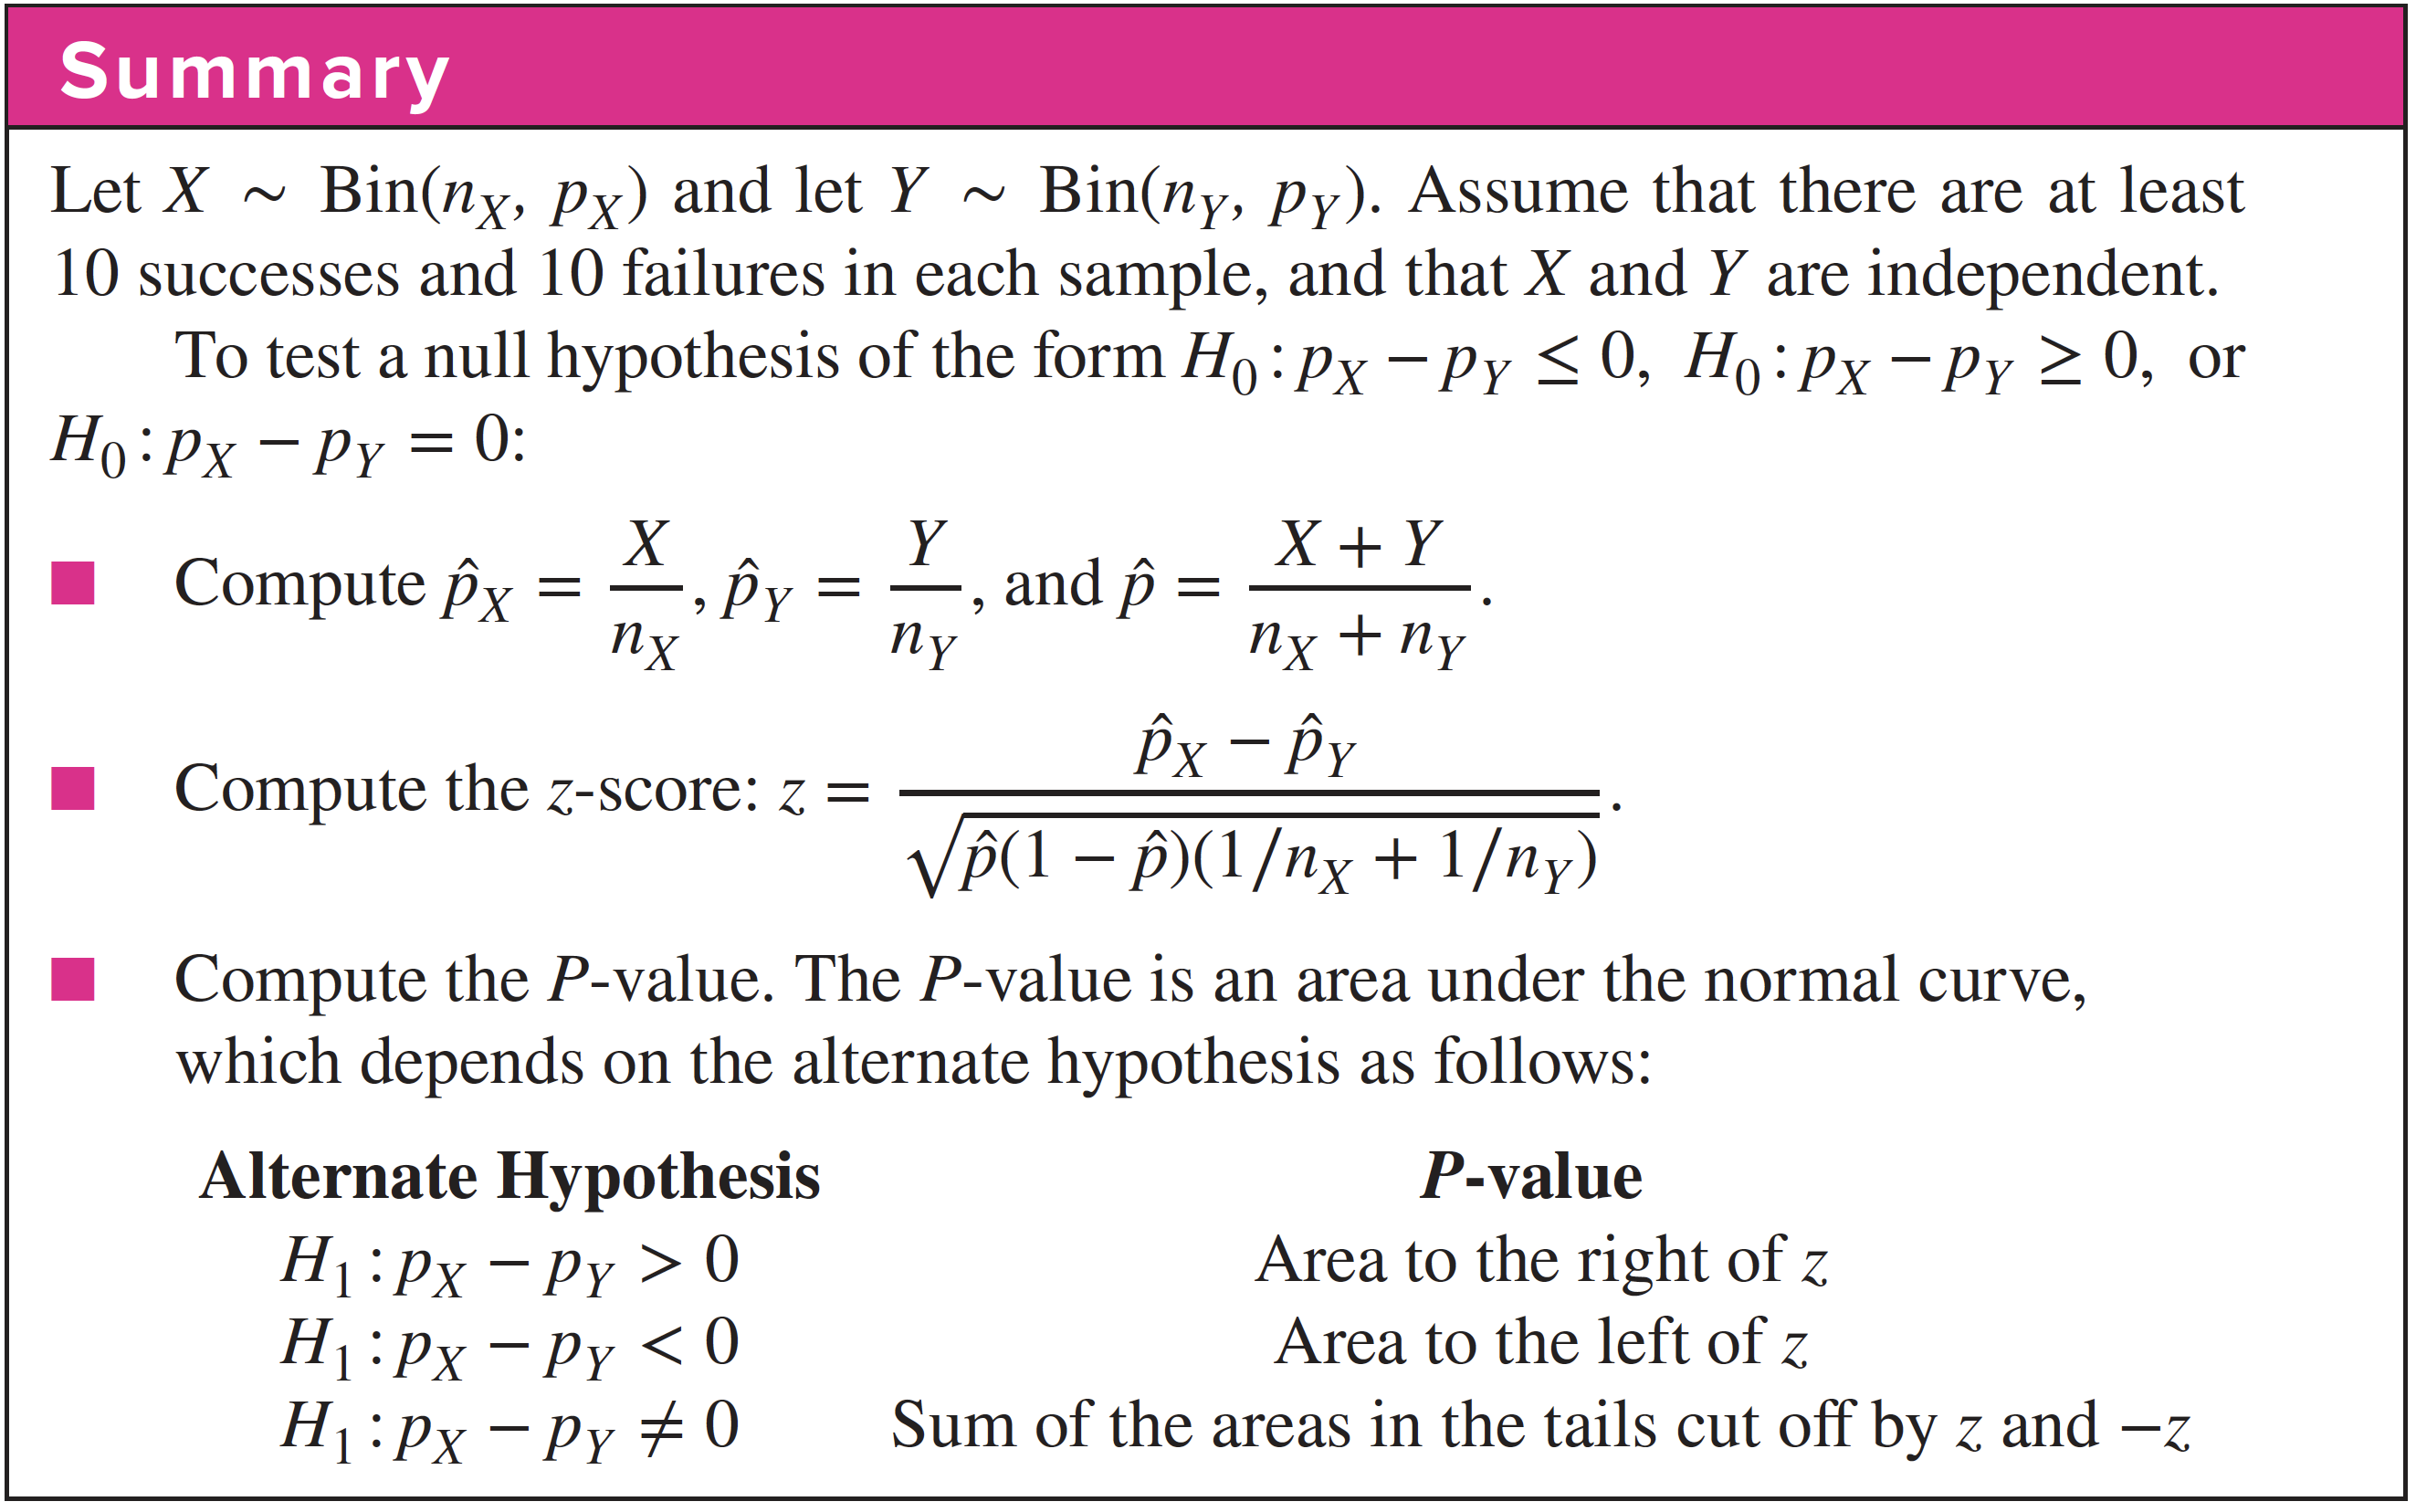
\includegraphics[width = 15cm]{Sections/Image/7_2summary.png}

\subsection{Small-Sample Inferences on the Difference Between Two Means}
Let \xotn be a random sample of size $n_X$ from a population with mean $\mu_X$ and standard deviation $\sigma_X$.\\
Let $Y_1, Y_2,...,Y_n$ be a random sample of size $n_Y$ from a population with mean $\mu_Y$ and standard deviation $\sigma_Y$.\\
If the two samples are independent, then a level of \cia CI for $\mu_X-\mu_Y$ is
\begin{equation*}
    \xbar-\bar{Y} \pm t_{v,\alphat} \sqrt{\frac{s_X^2}{n_X}+\frac{s_Y^2}{n_Y}}
\end{equation*}
The number of degrees of freedom v is given by:
\begin{equation*}
    v=\displaystyle \frac{\displaystyle(\frac{s_X^2}{n_X}+\frac{s_Y^2}{n_Y})^2}{\displaystyle\frac{(\frac{s_X^2}{n_X})^2}{n_X-1}+\displaystyle\frac{(\frac{s_Y^2}{n_Y})^2}{n_Y-1}}
\end{equation*}\\
Example:\\
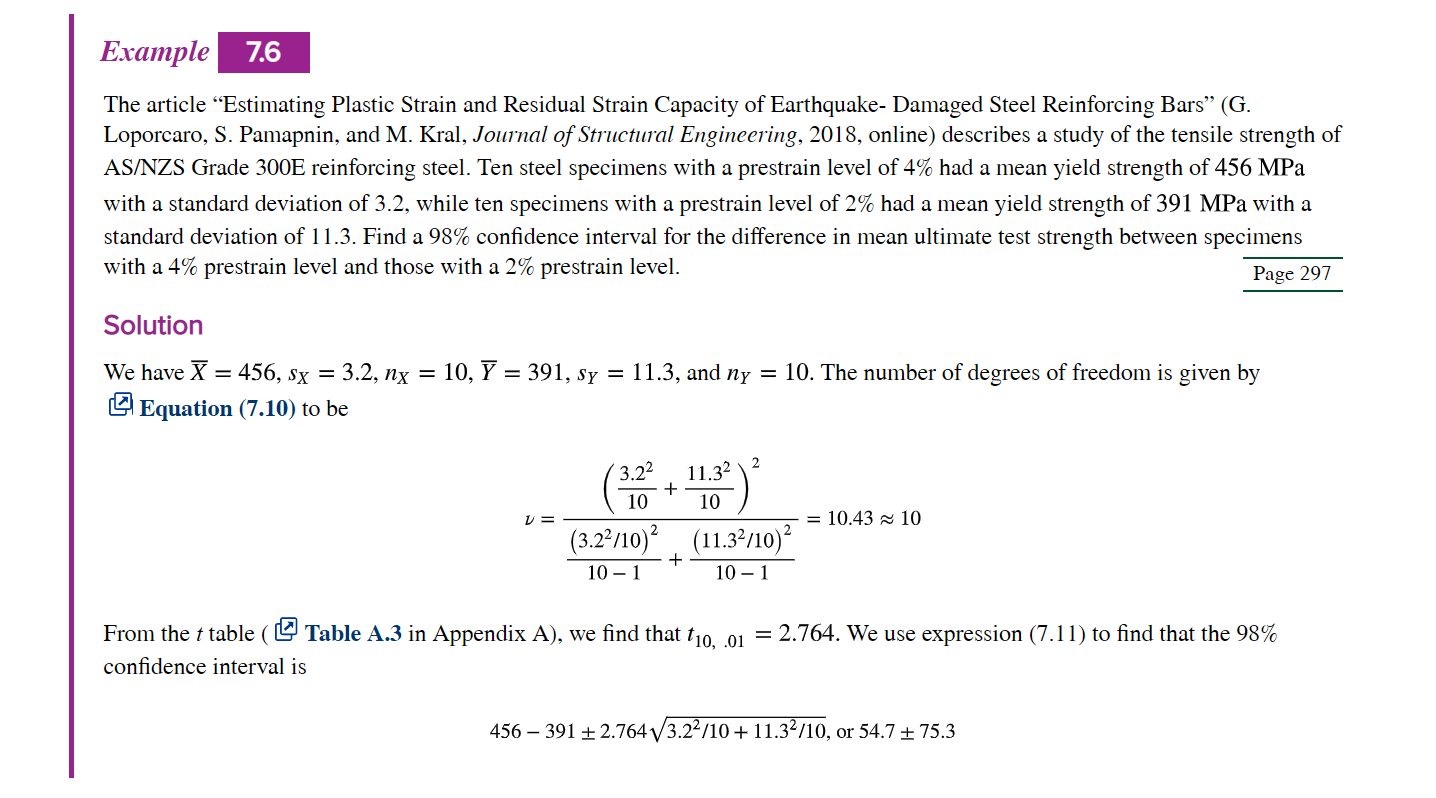
\includegraphics[width = 18cm]{Sections/Image/eg76.png}

\end{document}